\section{Enigma}

	\begin{frame}
		\begin{center}
			\LARGE{\textcolor{blue}{Enigma: storia, funzionamento ed analisi}}
		\end{center}
	\end{frame}
	
{ % all template changes are local to this group.
		\setbeamertemplate{navigation symbols}{}
		\begin{frame}[plain]
			\begin{tikzpicture}[remember picture,overlay]
			\node[at=(current page.center)] {
				\includegraphics[scale=0.74]{img/sfondo}
			};
			\end{tikzpicture}
		\end{frame}
	}	
	
	\subsection{Storia}
	
	\begin{frame}
		\frametitle{1918-1923}		
		\begin{itemize}
			\item Il \textcolor{blue}{23 Febbraio 1918}, l'ingegnere tedesco \tblue{Arthur Scherbius}, brevetta una "macchina cifrante a rotori"
			\item Nasce \tblue{ENIGMA}, una delle macchine cifranti più famose della storia
			\item Crea i primi prototipi e tenta di proporla alla milizia tedesca che al momento non è interessata
			\item Decide di fondare una propria azienda per produrre ENIGMA \textcolor{blue}{per scopi commerciali}. 
		\end{itemize}
	\end{frame}
	
	\begin{frame}
		\frametitle{1923-1932}			
		\begin{itemize}
			\item Nel \tblue{1923} vengono messe in commercio le prime macchine
			\item Incorporano una macchina da scrivere, sono \textcolor{blue}{molto pesanti} (circa 50kg) e \textcolor{blue}{poco pratiche} da utilizzare
			\item Non riscossero il successo previsto ma Scherbius continuò a lavorarci per migliorarle
		\end{itemize}
	\end{frame}

	\begin{frame}
		\frametitle{1923-1932}
		\begin{columns}
			\begin{column}{0.45\textwidth}
				\begin{figure}
					\centering
					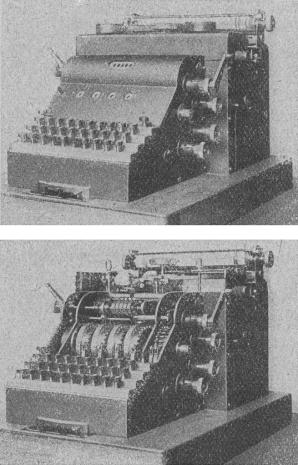
\includegraphics[scale=0.4]{img/A}
					\caption{ENIGMA modello A}
				\end{figure}
			\end{column}
			\begin{column}{0.45\textwidth}
				\begin{figure}
					\centering
					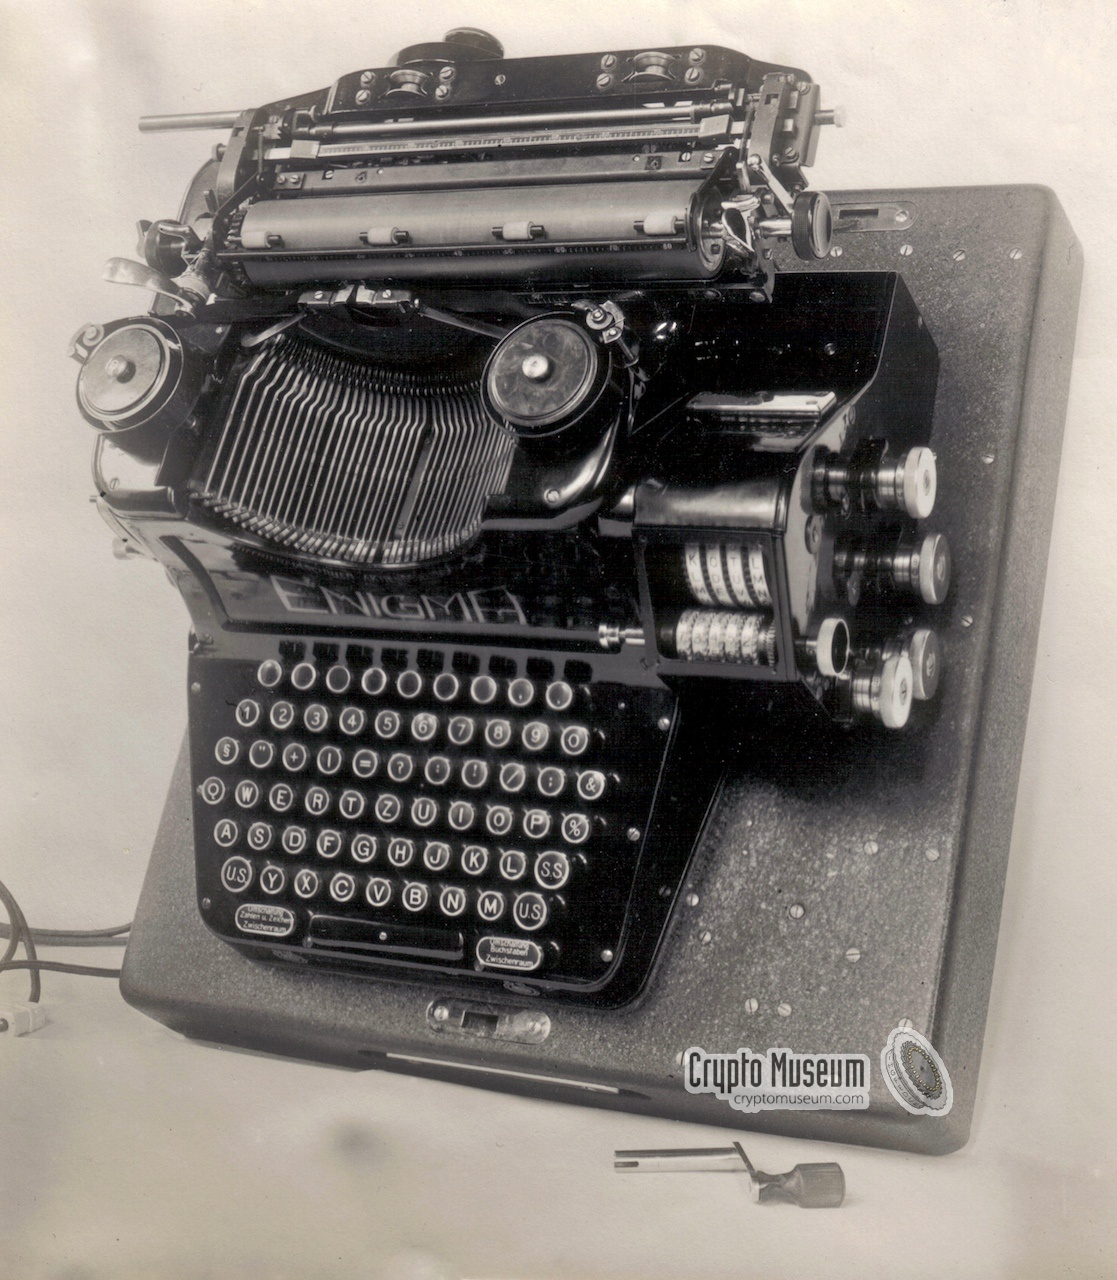
\includegraphics[scale=0.1]{img/B}
					\caption{ENIGMA modello B}
				\end{figure}
			\end{column}
		\end{columns}		
	\end{frame}
	
	\begin{frame}
		\frametitle{1923-1932}		
		\begin{itemize}
			\item Nel \tblue{1925} esce il modello C, il primo a presentare la \textcolor{blue}{lampboard}
			\item La marina si interessa alla macchina e nel \tblue{1926} la adotta ufficialmente (l'esercito lo farà solamente nel \tblue{1928})
			\item Nel \tblue{1932} viene introdotta la \textcolor{blue}{plugboard} e nasce la versione finale di ENIGMA, la \textcolor{blue}{ENIGMA-I}
			\item Da questo momento non è più disponibile in commercio ma viene riservata \textcolor{blue}{esclusivamente} a scopi militari
		\end{itemize}
	\end{frame}
	
	\begin{frame}
		\frametitle{1923-1932}
		\begin{columns}
			\begin{column}{0.45\textwidth}
				\begin{figure}
					\centering
					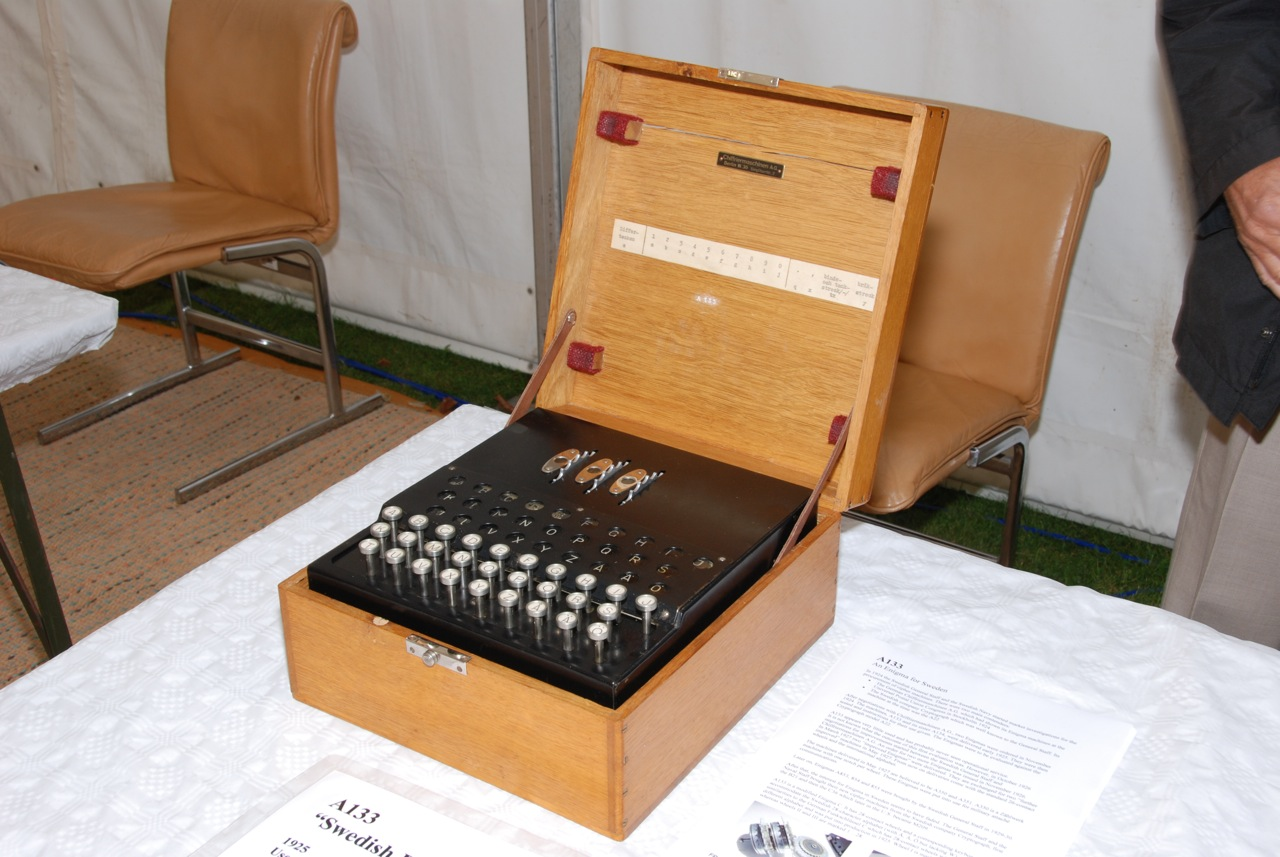
\includegraphics[width=\columnwidth]{img/C}
					\caption{ENIGMA modello C}
				\end{figure}
			\end{column}
			\begin{column}{0.45\textwidth}
				\begin{figure}
					\centering
					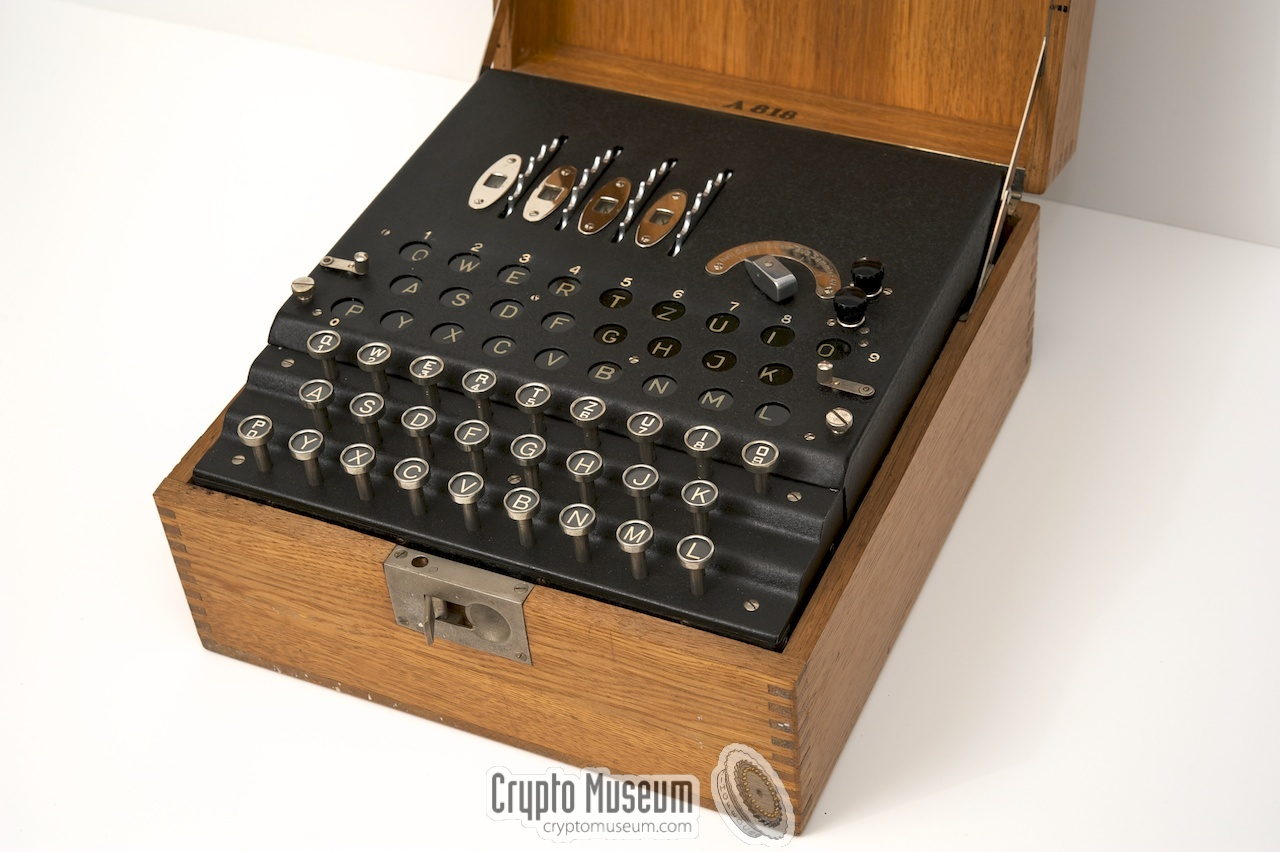
\includegraphics[width=\columnwidth]{img/D}
					\caption{ENIGMA modello D}
				\end{figure}
			\end{column}
		\end{columns}		
	\end{frame}
	
	\begin{frame}
		\frametitle{Dal 1932 alla caduta}		
		\begin{itemize}
			\item La marina e l'esercito \textcolor{blue}{continuano a lavorare su ENIGMA}, adattandola ognuno per i propri scopi e le due macchine presero strade completamente diverse
			\item Nel \tblue{1940} fece la sua apparizione \textcolor{blue}{ENIGMA-M3} l'ultima versione utilizzata dall'esercito per tutta la durata del conflitto.
			\item Da questo momento in avanti, ci riferiremo sempre a questo modello
		\end{itemize}
	\end{frame}
	
	\begin{frame}
		\frametitle{Dal 1932 alla caduta}		
		\begin{figure} [h]
			\centering
			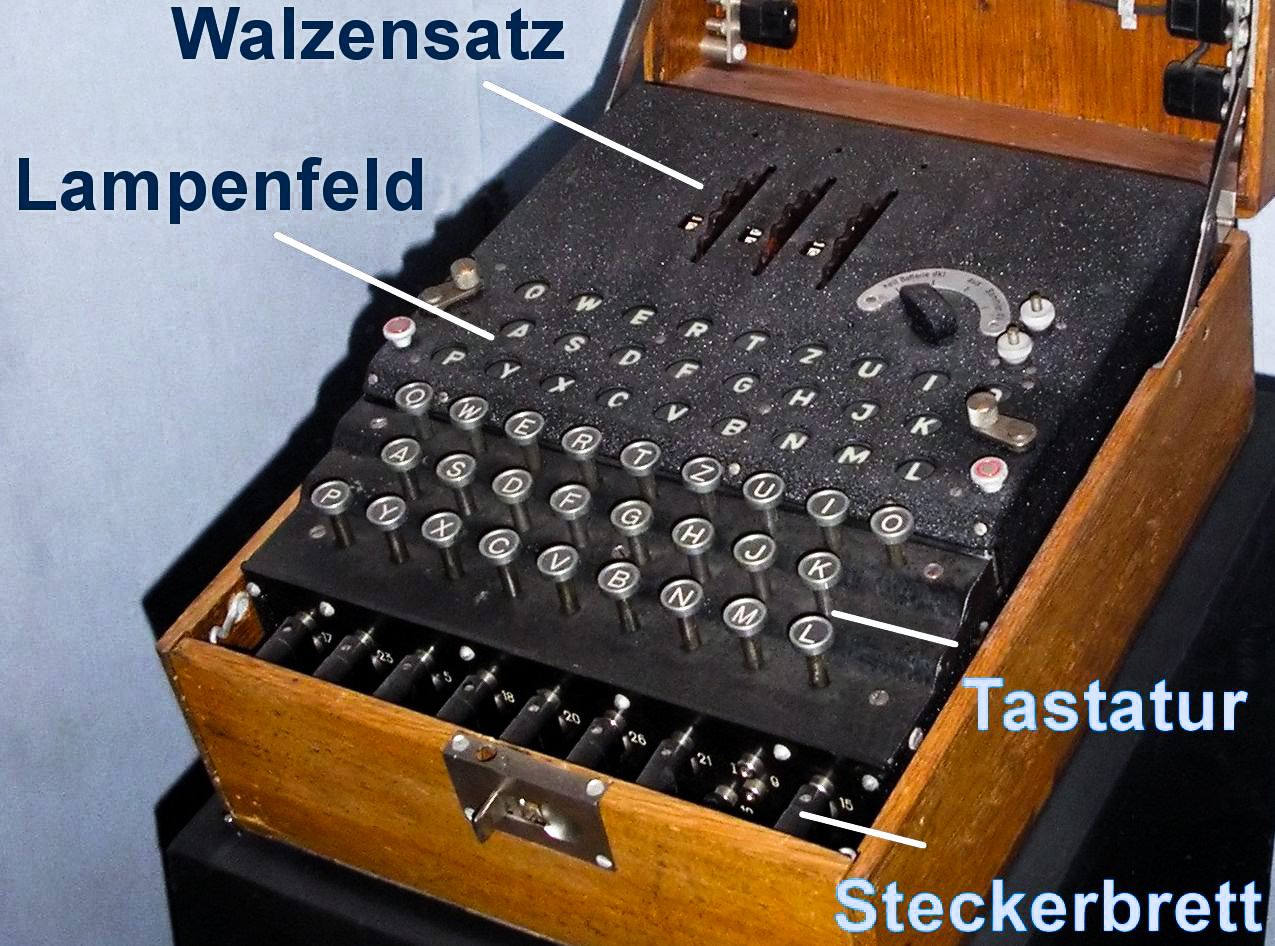
\includegraphics[scale = 0.5]{img/M3}
			\caption{ENIGMA modello M3}
		\end{figure}
	\end{frame}
	
	\subsection{Funzionamento}
	
	\begin{frame}
		\frametitle{Come funziona ENIGMA}
		\begin{itemize}
			\item ENIGMA implementa un \textcolor{blue}{cifrario a sostituzione polialfabetico}
			\item ENIGMA è un dispositivo \textcolor{blue}{elettromeccanico}
			\item Per spiegarne il funzionamento, seguiamo il percorso del \textcolor{blue}{segnale elettrico} al suo interno, dal momento in cui viene premuto un tasto fino all'accensione della lampadina
		\end{itemize}
	\end{frame}
	
	\begin{frame}
		\frametitle{Come funziona ENIGMA}
		\begin{figure}[h]
			\centering
			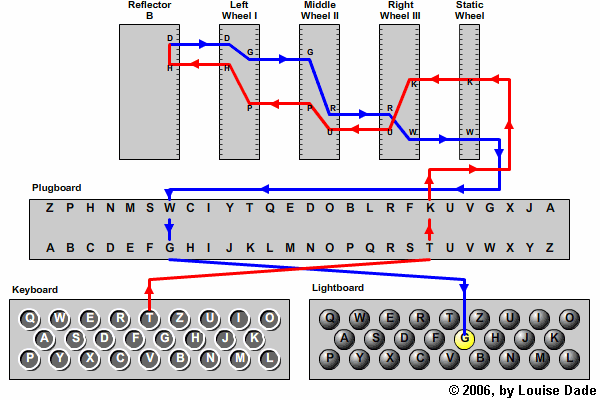
\includegraphics[scale=0.55]{img/wiring}
			\caption{Percorso seguito dal segnale all'interno di ENIGMA}
			\label{fig:wiring}
		\end{figure}
	\end{frame}
	
	\begin{frame}
		\frametitle{Come funziona ENIGMA}
		\begin{itemize}
			\item Analizziamo i vari componenti più in dettaglio
		\end{itemize}
	\end{frame}
	
	\begin{frame}
		\frametitle{Come funziona ENIGMA}
		\begin{figure}
			\centering
			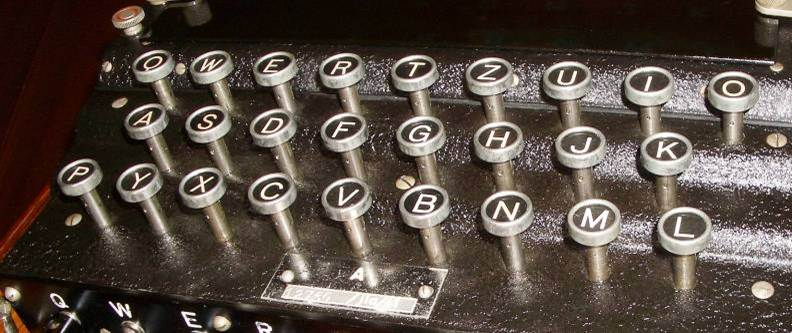
\includegraphics[scale=0.5]{img/keyboard}
			\caption{La tastiera di ENIGMA}
			\label{fig:keyboard}
		\end{figure}
	\end{frame}
	
	\begin{frame}
		\frametitle{Come funziona ENIGMA}
		\begin{figure}[h]
			\centering
			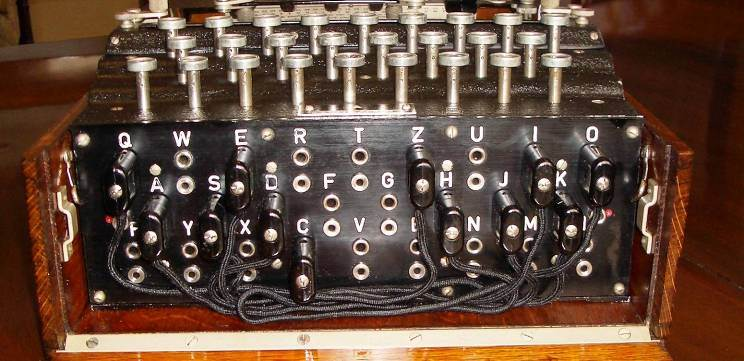
\includegraphics[scale=0.5]{img/plugboard}
			\caption{La plugboard di ENIGMA}
			\label{fig:plugboard}
		\end{figure}
	\end{frame}
	
	\begin{frame}
		\frametitle{Come funziona ENIGMA}
		\begin{columns}
			\begin{column}{0.5\textwidth}
				\begin{center}
					\begin{figure}
						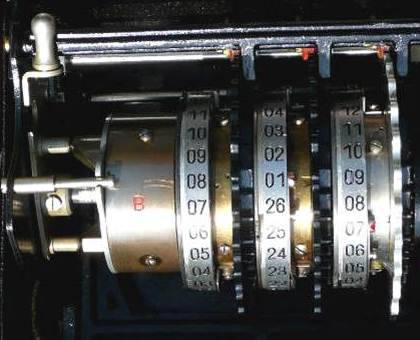
\includegraphics[width=\columnwidth]{img/rotors}
						\caption{Il reflector (a sinistra contrassegnato con una 'B' rossa) e i tre rotori}
					\end{figure}
				\end{center}
			\end{column}
			\begin{column}{0.5\textwidth}
				\begin{center}
					\begin{figure}
						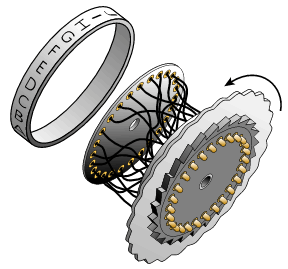
\includegraphics[width=\columnwidth]{img/rotorsexp}
						\caption{Modello di rotore}
					\end{figure}
				\end{center}
			\end{column}
		\end{columns}
	\end{frame}
	
	\begin{frame}
		\frametitle{Come funziona ENIGMA}
		\begin{figure}[h]
			\centering
			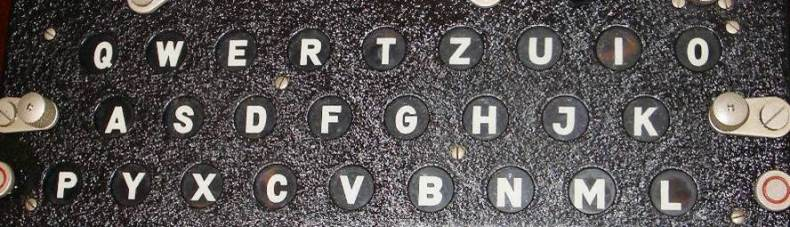
\includegraphics[scale=0.5]{img/lampboard}
			\caption{La lampboard}
			\label{fig:lampboard}
		\end{figure}
	\end{frame}

	\begin{frame}
		\frametitle{La chiave}
		\begin{columns}
			\begin{column}{0.5\textwidth}
				\begin{center}
					\begin{figure}
						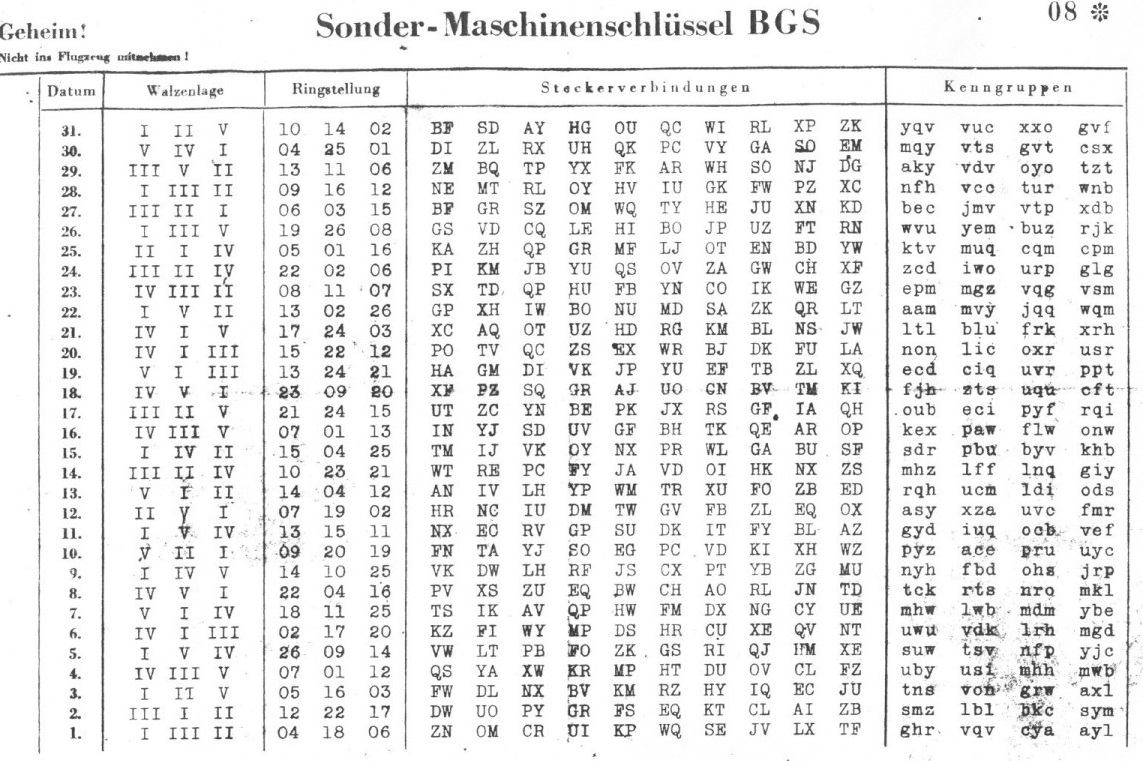
\includegraphics[width=\columnwidth]{img/enigmakeylist}
						\caption{Una pagina del libro delle chiavi}
					\end{figure}
				\end{center}
			\end{column}
			\begin{column}{0.5\textwidth}
				La \tblue{chiave} è formata da:
				\begin{itemize}
					\item I rotori scelti e il loro ordine
					\item La posizione iniziale di ogni rotore
					\item La configurazione della plugboard
					\item Dei caratteri di controllo per risalire alla data del messaggio
				\end{itemize}
			\end{column}
		\end{columns}
	\end{frame}
	
	\subsection{Analisi}
	
	\begin{frame}
		\frametitle{Analisi teorica}
		\begin{itemize}
			\item Configurazione della plugboard
		\end{itemize}
		\begin{figure}[h]
			\centering
			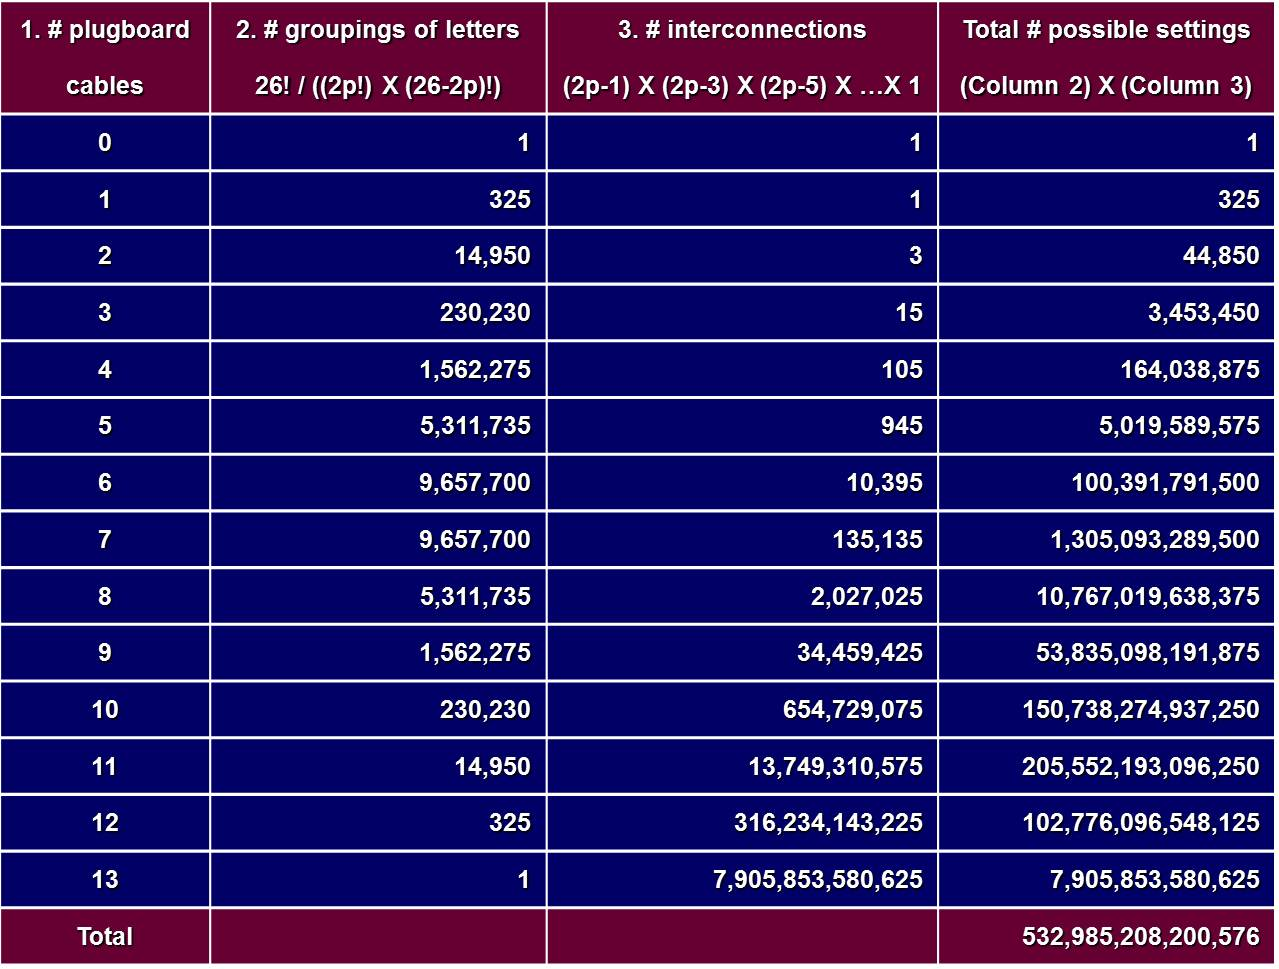
\includegraphics[scale=0.30]{img/plugboardsettings}
			\caption{Criteri possibili della plugboard e conseguenti combinazioni}
			\label{fig:plugboardsettings}
		\end{figure}		
	\end{frame}
	
	\begin{frame}
		\frametitle{Analisi teorica}
		\begin{itemize}
			\item Configurazione dei rotori
			\begin{itemize}
				\item Il cablaggio di ogni rotore poteva essere fatto in \textcolor{blue}{26!} combinazioni differenti
				\item Venivano utilizzati 3 rotori quindi le combinazioni diventano $$26!\cdot(26!-1)\cdot(26!-2)\approx \textcolor{blue}{6.5 \cdot 10^{78}}$$
				\item Ogni rotore poteva essere posizionato inizialmente in una qualunque delle 26 lettere ottenendo altre $\textcolor{blue}{26^3}$ combinazioni
				\item Il rotore più a destra avanza di una lettera ad ogni pressione della tastiera, il secondo e il terzo avanzano di una lettera dopo un giro completo del rotore alla rispettiva destra. Questo apporta ulteriori $(26 \cdot 26)$ \textcolor{blue}{676} combinazioni
			\end{itemize}
		\end{itemize}
	\end{frame}
	
	\begin{frame}
		\frametitle{Analisi teorica}
		\begin{itemize}
			\item Configurazione del reflector
			\begin{itemize}
				\item Il reflector scambia \textcolor{blue}{coppie} di lettere 
				\item La lettera 'A' può essere scambiata con una qualunque delle 25 lettere rimanenti, la lettera successiva con le rimanenti 23 e così via
				\item Il risultato è lo stesso di quello ottenuto utilizzando una plugboard a tredici cavi ed è pari a $\textcolor{blue}{7,905,853,580,625}$ combinazioni.
			\end{itemize}
		\end{itemize}
	\end{frame}
	
	\begin{frame}
		\frametitle{Analisi teorica}
		\begin{itemize}
			\item Limite teorico totale
			\begin{itemize}
				\item Il limite teorico totale di combinazioni si ottiene moltiplicando i risultati fin qui ottenuti
				\item Tale numero è dell'ordine di $\textcolor{blue}{3.28 \cdot 10^{114}}$
				\item Il numero di atomi presenti in tutto l'universo osservabile è nell'ordine di $\textcolor{blue}{10^{80}}$.
			\end{itemize}
		\end{itemize}
	\end{frame}
	
	\begin{frame}
		\frametitle{Analisi pratica}
		\begin{itemize}
			\item Venivano utilizzati \tblue{sempre} dieci cavi per la plugboard e questo riduce le possibili configurazioni a $\textcolor{blue}{150,738,274,937,250}$
			\item Vennero costruiti solamente 5 rotori quindi, selezionandone 3 tra questi 5 otteniamo $(5 \cdot 4 \cdot 3)$ \textcolor{blue}{60} combinazioni.
			\item Le possibili posizioni iniziali dei rotori e il sistema di avanzamento resta immutato e quindi si hanno $\textcolor{blue}{17,576}$ e \textcolor{blue}{676} combinazioni.
			\item Il reflector era fisso e noto quindi non apporta combinazioni.
		\end{itemize}
	\end{frame}
	
	\begin{frame}
		\frametitle{Analisi pratica}
		\begin{itemize}
			\item Il prodotto di queste quantità si attesta intorno a $\textcolor{blue}{1.07 \cdot 10^{23}}$(molto inferiore rispetto al limite teorico ma comunque incredibilmente grande)
			\item Supponendo di avere 100.000 operatori in grado di verificare una combinazione al secondo, servirebbe circa \tblue{due volte l'età dell'universo} per provarle tutte.
			\item Grazie al lavoro di Turing si stima che la guerra è stata accorciata di due anni
		\end{itemize}
	\end{frame}